\section{Théorèmes limites}
Everything up to here has been about one variable aléatoire, or finitely many at
a time: its loi, its moments, its fonction caractéristique, the loi of a vector
built from it. Ce chapitre porte sur deux résultats fondamentaux de convergence
de suites de variables aléatoires : la loi des grands nombres et le théorème
central limite --- the two results the whole construction was built for. The loi
forte des grands nombres says that an empirical mean settles on the espérance,
and the théorème central limite that the error it makes on the way there is
Gaussian.\\
Both are statements that a sequence $X_{1}, X_{2}, \dots$ converges to
something, so both need a notion of convergence for variables aléatoires, and
there is more than one. A variable aléatoire is a function on $\Omega$, so one
can ask for convergence of the functions --- pointwise, for almost every
$\omega$ --- and that is the strongest thing to ask. Or one can forget $\Omega$
entirely and ask only that the \emph{lois} converge, which is much weaker and is
exactly what the théorème central limite delivers. Nous commençons par définir
deux notions usuelles de convergence d'une suite de variables aléatoires : la
convergence presque sûre et la convergence en loi. The first two subsections
below set them up and relate them; the last three are the theorems.

\begin{remark}
  D'autres notions de convergence existent, comme la convergence en
  probabilité, mais ne sont pas abordées
  dans ce cours --- convergence in $L^{p}$ is another. Convergence en
  probabilité is carried here anyway, marked as an addition, for the reason
  given at the end of the first subsection.
\end{remark}

\subsection{Convergence presque sûre}
Two French abbreviations run through this chapter, both already in use.
\textit{p.s.} is the probabilistic name for \textit{p.p.} from chapter 2,
specialised to a mesure that happens to be a probability --- the exceptional
set is $\prob$-négligeable rather than merely $\lambda$-négligeable, but nothing
else changes.\\
For an i.i.d.\ sequence both halves of the abbreviation are used in the proofs
below, and they are used differently --- indépendance gives the factorisation of
a fonction caractéristique or the vanishing of a cross term, and being
identiquement distribuées gives the single loi that the limit is expressed in
terms of. A sequence can have one without the other, and then neither theorem in
this chapter applies.

\begin{notation}
  Throughout, $X_{1}, X_{2}, \dots$ is a sequence of variables aléatoires réelles
  on a common espace de probabilité $(\Omega, \mathcal{F}, \prob)$, and
  $S_{n} = \sum_{i=1}^{n} X_{i}$ is its sequence of partial sums. That the space
  is common matters for convergence presque sûre, which compares
  $X_{n}(\omega)$ with $X(\omega)$ for the same $\omega$, and not at all for
  convergence en loi, which never looks at $\omega$.\\
  Two Greek letters are kept apart: $\varphi$ is a fonction caractéristique ---
  $\varphi_{X}$, $\varphi_{n}$, or a bare $\varphi$ for the limit's --- and
  $\phi$ is always a fonction test, bounded and continuous where convergence en
  loi is being tested, mesurable and non-negative where the théorème de
  transfert is being applied. A continuous map applied to a sequence is written
  $g$.
\end{notation}

La notion de convergence la plus forte est une convergence simple, valable pour
presque toute réalisation $\omega$: simple pointwise convergence of the
functions $X_{n} : \Omega \to \reals$, asked for not at every realisation but at
almost every one.

\begin{definition}[Convergence presque sûre (\textit{almost-sure convergence})]
  On dit qu'une suite de variables aléatoires réelles $X_{1}, X_{2}, \dots$
  converge \textbf{presque sûrement} vers une variable aléatoire réelle $X$ si
  la suite $X_{1}(\omega), X_{2}(\omega), \dots$ converge
  vers $X(\omega)$ pour presque tout $\omega \in \Omega$ :
  \[
    \prob\left(\left\{\omega \in \Omega : \lim_{n \to +\infty} X_{n}(\omega)
      = X(\omega)\right\}\right) = 1 .
  \]
\end{definition}

\begin{notation}
  On utilise la notation :
  \[
    X_{n} \cvas X .
  \]
\end{notation}

The set appearing in the definition is mesurable --- it is
$\bigcap_{k \geq 1} \bigcup_{N \geq 1} \bigcap_{n \geq N}
\{|X_{n} - X| \leq 1/k\}$, a countable combination of événements --- so asking
for its probability is legitimate. What the definition does \emph{not} require
is convergence at every $\omega$, and in most applications there is a genuine
exceptional événement: the binary-digit example below has one, and it contains
the dyadic rationals, whose expansions are eventually constant. It is
$\prob$-négligeable, but not for the cheap reason of being countable --- it is
not countable.

\begin{prop}
  Si $X_{n} \cvas X$, alors $g(X_{n}) \cvas g(X)$ pour toute fonction
  continue $g$.
\end{prop}

\begin{proof}
  Soit $\omega \in \Omega$ tel que $\lim_{n} X_{n}(\omega) = X(\omega)$. Pour
  toute fonction continue $g$,
  $\lim_{n} g(X_{n}(\omega)) = g(X(\omega))$, by continuity at the point
  $X(\omega)$. The événement on which $g(X_{n})$ converges to $g(X)$ therefore
  contains the événement on which $X_{n}$ converges to $X$. On a donc :
  \[
    \prob\left(\lim_{n} g(X_{n}) = g(X)\right)
      \geq \prob\left(\lim_{n} X_{n} = X\right) = 1 .
  \]
\end{proof}

That one line is worth remembering as a move rather than as a result.
Convergence presque sûre is convergence of numbers at a fixed $\omega$, so
anything true of convergent sequences of reals transfers to it by intersecting
événements of probability $1$ --- countably many of which still intersect to an
événement of probability $1$. It is why the loi forte can be composed with a
logarithm or an exponential below without further work.

\subsubsection{Convergence en probabilité, un complément}
The next definition is \emph{not} part of the course. The course defines
convergence presque sûre and convergence en loi, and names convergence en
probabilité only to say that it is not treated --- so nothing about it is ever
defined or proved in it. It is carried here for one reason: it sits between
the two modes the course does define, it is assumed wherever it turns up, and a
problem on this syllabus may well supply the definition inline before asking
for the implication below, precisely because the course does not.

\begin{definition}[Convergence en probabilité (\textit{convergence in probability}) --- hors programme]
  A sequence of variables aléatoires réelles $X_{1}, X_{2}, \dots$ converges
  \textbf{en probabilité} to a variable aléatoire réelle
  $X$ if
  \[
    \forall a > 0, \qquad \lim_{n \to +\infty} \prob(|X_{n} - X| > a) = 0 .
  \]
  This is written $X_{n} \cvP X$.
\end{definition}

\begin{prop}[Hors programme]
  If $X_{n} \cvas X$, then $X_{n} \cvP X$.
\end{prop}

\begin{proof}
  Fix $a > 0$ and write the probability as an integral of an indicator:
  \[
    \prob(|X_{n} - X| > a) = \int_{\Omega} \indic_{\{|X_{n} - X| > a\}}
      \, d\prob .
  \]
  On the événement of probability $1$ where $X_{n}(\omega) \to X(\omega)$, one
  has $|X_{n}(\omega) - X(\omega)| \leq a$ for all $n$ large enough, so the
  integrand tends to $0$ \textit{p.s.}. It is bounded by the constant function
  $1$, which is integrable because $\prob(\Omega) = 1$ is finite, so convergence
  dominée applies and the integral tends to $0$.
\end{proof}

\begin{remark}
  The domination is available only because the mesure is finite --- the
  constant $1$ is not integrable for the mesure de Lebesgue on $\reals$ --- so
  this is one of the few places where the normalisation $\prob(\Omega) = 1$ does
  real work rather than bookkeeping.
\end{remark}

\begin{remark}
  The converse is false: a single indicator window of width $1/n$ sliding
  cyclically around $[0,1]$ has $\prob(|X_{n}| > a) = 1/n \to 0$, so
  $X_{n} \cvP 0$, while every $\omega$ is hit infinitely often and
  $X_{n}(\omega)$ converges for no $\omega$ at all.
\end{remark}

\subsection{Convergence en loi}
The second notion forgets the univers. Comme son nom l'indique, elle ne concerne
que les \emph{lois} des variables aléatoires impliquées, et non leur
réalisation: the variables need not even be defined on the same espace de
probabilité, and nothing is being compared $\omega$ by $\omega$. What is
compared is the sequence of fonctions de répartition.

\begin{definition}[Convergence en loi (\textit{convergence in distribution})]
  On dit qu'une suite de variables aléatoires réelles $X_{1}, X_{2}, \dots$
  converge \textbf{en loi} vers une variable aléatoire réelle $X$ si leurs
  fonctions de répartition $F_{1}, F_{2}, \dots$ convergent vers sa fonction de
  répartition $F$ en tout point de continuité de celle-ci :
  \[
    \forall x \text{ where } F \text{ is continuous}, \qquad
      \lim_{n \to +\infty} F_{n}(x) = F(x) .
  \]
\end{definition}

\begin{notation}
  On utilise la notation :
  \[
    X_{n} \cvL X .
  \]
  Comme cette notion de convergence s'applique aux lois, on pourra également
  l'écrire comme tel, par exemple $X_{n} \cvL \mathcal{N}(0,1)$: the right-hand
  side may be a loi rather than a variable, and this means that the loi limite
  is the loi normale centrée réduite.
\end{notation}

The restriction to continuity points of $F$ is not a technical nicety appended
to make some proof work --- it is the content of the definition. Requiring
$F_{n}(x) \to F(x)$ at \emph{every} $x$ would break the two most natural
examples of convergence to a constant, and a version of the definition without
the restriction is simply wrong.

\begin{example}[A Gaussian collapsing onto a point]
  Soit une suite de variables aléatoires avec $X_{n} \sim \mathcal{N}(0, 1/n)$
  pour tout $n \geq 1$. The variance shrinks to $0$ and the loi concentrates at
  the origin:
  \[
    \forall x, \qquad \lim_{n \to +\infty} \prob(X_{n} \leq x) =
      \begin{cases}
        0 & \text{for } x < 0 , \\
        1 & \text{for } x > 0 ,
      \end{cases}
  \]
  which is the fonction de répartition of the constant variable aléatoire
  $0$ at every $x \neq 0$. Cette suite converge donc en loi vers zéro:
  $X_{n} \cvL 0$. At $x = 0$ itself the limit fails:
  by symmetry $F_{n}(0) = 1/2$ for every $n$, while $F(0) = 1$. The single point
  where the convergence breaks down is the single discontinuity of $F$, and the
  definition excludes exactly it.
\end{example}

\begin{example}[A deterministic sequence, converging en loi to a constant]
  The same phenomenon with no randomness at all. Let $X_{n}$ be deterministic and
  equal to $1/n$, and $X$ deterministic and equal to $0$. Then
  \[
    F_{n}(x) = \indic_{\{x \geq 1/n\}}, \qquad
    F(x) = \indic_{\{x \geq 0\}} ,
  \]
  and $X_{n} \to X$ in the most literal sense available --- the numbers converge.
  For $x < 0$, $F_{n}(x) = 0 = F(x)$ for every $n$; for $x > 0$,
  $F_{n}(x) = 1 = F(x)$ as soon as $n > 1/x$. But at $x = 0$,
  $F_{n}(0) = 0$ for every $n$, while $F(0) = 1$, and the sequence $F_{n}(0)$
  does not converge to $F(0)$. Without the continuity-point restriction the
  definition would refuse to call $1/n \to 0$ a convergence en loi, which is
  absurd; with it, the one bad point is the one jump of $F$ and is discarded.
\end{example}

The figure draws that second example. The two fonctions de répartition
agree everywhere except on the interval $[0, 1/n)$, which shrinks to nothing, and
the one point where they refuse to meet in the limit is the jump of $F$.

\begin{figure}[h!]
  \centering
  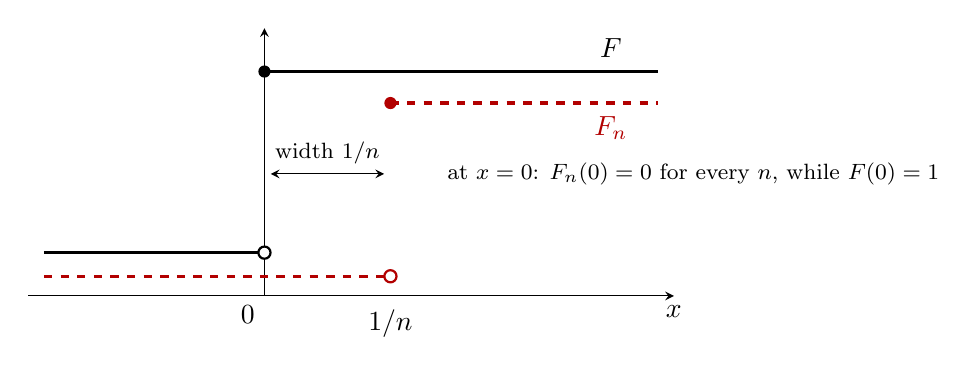
\begin{tikzpicture}[>=stealth, scale=1.0]
    % axes
    \draw[->] (-3.0,0) -- (5.2,0) node[below] {$x$};
    \draw[->] (0,0) -- (0,3.4);
    \node[below left] at (0,0) {$0$};
    % F : value 0 up to x = 0, value 1 after
    \draw[very thick] (-2.8,0.55) -- (-0.02,0.55);
    \draw[very thick] (0,2.85) -- (5.0,2.85);
    \fill (0,2.85) circle (2.2pt);
    \draw[thick,fill=white] (0,0.55) circle (2.2pt);
    \node[above] at (4.4,2.9) {$F$};
    % F_n : the same, jumping at 1/n instead
    \draw[very thick,dashed,red!70!black] (-2.8,0.25) -- (1.58,0.25);
    \draw[very thick,dashed,red!70!black] (1.6,2.45) -- (5.0,2.45);
    \fill[red!70!black] (1.6,2.45) circle (2.2pt);
    \draw[thick,fill=white,draw=red!70!black] (1.6,0.25) circle (2.2pt);
    \node[below,red!70!black] at (4.4,2.4) {$F_{n}$};
    \node[below] at (1.6,-0.05) {$1/n$};
    % the stretch on which they disagree
    \draw[<->] (0.08,1.55) -- (1.52,1.55);
    \node[above] at (0.8,1.55) {\footnotesize width $1/n$};
    \node[anchor=west,font=\footnotesize] at (2.2,1.55)
      {at $x = 0$: $F_{n}(0) = 0$ for every $n$, while $F(0) = 1$};
  \end{tikzpicture}\\[2mm]
  {\footnotesize The two fonctions en escalier take the values $0$ and $1$; they
   are drawn at slightly different heights only to keep them apart.}
\end{figure}

Le résultat suivant, dont la preuve est omise, donne deux autres façons de
caractériser la convergence en loi, and they are what make it usable: the first
replaces fonctions de répartition by fonctions test, and the second replaces them
by fonctions caractéristiques, which is the bridge back to the previous chapters
and the engine of the théorème central limite.

\begin{theorem}[Trois caractérisations de la convergence en loi]
  Soit $X_{1}, X_{2}, \dots$ une suite de variables aléatoires réelles, de
  fonctions caractéristiques respectives $\varphi_{1}, \varphi_{2}, \dots$, et
  $X$ une variable aléatoire réelle, de fonction caractéristique $\varphi$. Les
  propositions suivantes sont équivalentes :
  \begin{enumerate}
    \item La suite $X_{1}, X_{2}, \dots$ converge en loi vers $X$.
    \item Pour toute fonction \emph{continue bornée} $\phi$,
      \[
        \lim_{n \to +\infty} \expec(\phi(X_{n})) = \expec(\phi(X)) .
      \]
    \item Pour tout $t \in \reals$,
      \[
        \lim_{n \to +\infty} \varphi_{n}(t) = \varphi(t) .
      \]
  \end{enumerate}
\end{theorem}

\begin{remark}
  Both hypotheses on the fonction test in branch 2 are needed. Bounded, because
  $\expec(\phi(X_{n}))$ must exist without any integrability assumption on
  $X_{n}$ --- and the theorem is stated for arbitrary sequences, with no moments
  assumed. Continuous, because the definition tolerates failure at the
  discontinuity points of $F$, and a discontinuous fonction test can be built to
  sit exactly on one of them: taking $\phi = \indic_{(-\infty, 0]}$ in the
  deterministic example above gives $\expec(\phi(X_{n})) = 0$ for every $n$
  and $\expec(\phi(X)) = 1$.
\end{remark}

\begin{remark}
  Branch 3 is the reason the fonction caractéristique chapter comes before this
  one. It converts a question about lois --- objects with no
  arithmetic ---
  into a question about pointwise convergence of a sequence of functions on
  $\reals$, and fonctions caractéristiques of sums of independent variables
  multiply. Pointwise convergence, with no uniformity asked for anywhere, is all
  that is required. The full statement of the corresponding converse (Lévy's
  theorem, requiring the limit to be continuous at $0$) is not part of this
  course: here the limit $\varphi$ is always given in advance as the
  fonction caractéristique of an actual variable aléatoire, which is what
  branch 3 presupposes.
\end{remark}

Convergence en loi can also be read off densités when they exist, and the proof
is one application of convergence dominée followed by one application of the
theorem above.

\begin{prop}[Densités convergeant presque partout]
  Soit $X_{1}, X_{2}, \dots$ une suite de variables aléatoires réelles, de
  densités respectives $f_{1}, f_{2}, \dots$, et $X$ une variable aléatoire
  réelle, de densité $f$. Si la suite $(f_{n})_{n \geq 1}$ converge presque
  partout vers $f$, alors la suite $X_{1}, X_{2}, \dots$ converge en loi
  vers $X$.
\end{prop}

\begin{proof}
  Pour toute fonction continue bornée $\phi$, the théorème de transfert gives
  \[
    \expec(\phi(X_{n})) = \int \phi(x) f_{n}(x) \, dx
      \; \longrightarrow \; \int \phi(x) f(x) \, dx = \expec(\phi(X)) ,
  \]
  par convergence dominée: the integrands converge
  \textit{p.p.}, since $f_{n} \to f$ \textit{p.p.} and $\phi$ is fixed, and
  they are bounded in modulus by $\|\phi\|_{\infty} f_{n}$. Le résultat est
  alors une conséquence du théorème précédent --- its branch 2.
\end{proof}

\begin{remark}
  The domination needs care: the bound $\|\phi\|_{\infty} f_{n}$ moves with
  $n$, so it is not a fixed dominating function and the argument as written is a
  sketch. The repair leans on a standard result the course neither states nor
  proves (Scheffé's lemma): $f_{n} \to f$ \textit{p.p.}, all non-negative of
  integral $1$, forces $\int |f_{n} - f| \to 0$, and then
  $|\expec(\phi(X_{n})) - \expec(\phi(X))| \leq \|\phi\|_{\infty}
  \int |f_{n} - f| \to 0$, with no domination needed at all.
\end{remark}

\begin{remark}
  The implication runs one way only. Convergence en loi does not give
  convergence of densités, and the loi limite need not even have a densité: the
  two examples above converge en loi to a constant, whose loi
  is a mesure de Dirac
  with no densité at all. Convergence of densités is a genuinely stronger
  hypothesis, which is why it is stated as a sufficient condition and not as a
  characterisation.
\end{remark}

The two notions of convergence are now related. La convergence presque sûre est
plus forte que la convergence en loi :

\begin{theorem}[La convergence presque sûre implique la convergence en loi]
  Soit $X_{1}, X_{2}, \dots$ une suite de variables aléatoires réelles :
  \[
    X_{n} \cvas X \quad \Longrightarrow \quad X_{n} \cvL X .
  \]
\end{theorem}

\begin{proof}
  Pour toute fonction continue bornée $\phi$, on a par continuité (the
  stability of convergence presque sûre under a continuous map) :
  \[
    \phi(X_{n}) \cvas \phi(X) .
  \]
  La fonction $\phi$ étant bornée, the sequence $\phi(X_{n})$ is dominated by
  the constant $\|\phi\|_{\infty}$, which is integrable for the finite mesure
  $\prob$; on a donc par le théorème de convergence dominée :
  \[
    \lim_{n \to +\infty} \expec(\phi(X_{n})) = \expec(\phi(X)) .
  \]
  Le résultat découle du théorème des trois caractérisations --- this is its
  branch 2 --- so $X_{n} \cvL X$.
\end{proof}

\begin{prop}
  Si $X_{n} \cvL X$, alors $g(X_{n}) \cvL g(X)$ pour toute fonction
  continue $g$.
\end{prop}

\begin{proof}
  Pour toute fonction continue bornée $\phi$, la fonction $\phi \circ g$ est
  elle-même continue bornée --- bounded since $\phi$ is. Par le théorème des
  trois caractérisations (branch 2), applied to $X_{n} \cvL X$,
  \[
    \lim_{n \to +\infty} \expec(\phi \circ g(X_{n}))
      = \expec(\phi \circ g(X)) .
  \]
  As this holds for every bounded continuous $\phi$, l'application de ce même
  théorème, read in the other direction, implique que $g(X_{n}) \cvL g(X)$.
\end{proof}

\begin{remark}
  Both stability results are used in the same shape: prove a convergence for the
  easiest transform of the sequence --- usually a logarithm, which turns a
  product into a sum the limit theorems can reach --- then push it through the
  exponential. The examples below do this twice.
\end{remark}

\subsubsection{Liens entre les modes de convergence}
Collecting the implications, with the mode that is not part of the course drawn
dashed:

\begin{figure}[h!]
  \centering
  \begin{tikzpicture}[>=stealth, node distance=12mm and 26mm]
    \node[draw, very thick, rounded corners, inner sep=6pt] (as)
      {$X_{n} \cvas X$};
    \node[draw, dashed, rounded corners, inner sep=6pt, right=of as] (p)
      {$X_{n} \cvP X$};
    \node[draw, very thick, rounded corners, inner sep=6pt, right=of p] (l)
      {$X_{n} \cvL X$};
    \draw[->, very thick] (as) -- node[above,font=\footnotesize] {conv.\ dom.} (p);
    \draw[->, dashed] (p) -- node[above,font=\footnotesize] {not proved here} (l);
    \draw[->, very thick] (as.south) .. controls +(0,-1.2) and +(0,-1.2) ..
      node[below,font=\footnotesize]
      {conv.\ dom.\ on bounded continuous tests} (l.south);
    \node[below=18mm of p, align=center, font=\footnotesize]
      {the dashed box and the dashed arrow are the addition ---\\
       the course defines only the two solid modes};
  \end{tikzpicture}
\end{figure}

\begin{remark}
  None of the arrows reverses. The sliding window above converges en
  probabilité and not presque sûrement; and with $X$ of loi normale centrée
  réduite and $X_{n} = -X$ for every $n$, $X_{n} \cvL X$ holds trivially while
  $|X_{n} - X| = 2|X|$ never gets small. The one partial converse worth knowing
  belongs to the addition and is stated, not proved, here: convergence en loi
  \emph{to a constant} does imply convergence en probabilité to that constant.
\end{remark}

\subsection{Loi forte des grands nombres}
La \textbf{loi forte des grands nombres} (\textit{strong law of large numbers})
régit la limite de la moyenne empirique d'une suite de variables aléatoires
i.i.d. La seule condition est que ces variables aléatoires aient une espérance
--- no variance, no higher moment, nothing else. On parle de loi \emph{forte}
car elle implique la convergence presque sûre: a weak law would conclude only
convergence en probabilité.

\begin{theorem}[Loi forte des grands nombres]
  Pour toute suite $X_{1}, X_{2}, \dots$ de variables aléatoires réelles
  i.i.d.\ \emph{ayant une espérance},
  \[
    \frac{1}{n} \sum_{i=1}^{n} X_{i} \cvas \expec(X_{1}) .
  \]
\end{theorem}

\begin{remark}
  The hypothesis is exactly ``i.i.d.\ with an espérance'', that is,
  $\expec(|X_{1}|) < +\infty$. It is \emph{not} ``with a finite variance'': that
  stronger hypothesis belongs to the weak law and to the proof carried below,
  and importing it into the statement would weaken the theorem for no gain. The
  distinction is not academic --- the Cauchy example at the end of this
  subsection is a sequence with no espérance, and for it the theorem has
  nothing to say and the empirical mean genuinely fails to settle.
\end{remark}

\begin{proof}
  \textit{On donne une preuve partielle, dans le cas où les variables
  aléatoires ont un moment d'ordre 4.}\\
  Quitte à recentrer ces variables, on suppose que leur espérance est nulle,
  $\expec(X_{1}) = 0$, et on note
  $S_{n} = \sum_{i=1}^{n} X_{i}$.\\
  \textbf{Step 1: a bound on the moment d'ordre 4 of $S_{n}$.} Expand
  $S_{n}^{4}$ and take espérances. Indépendance makes every term containing a
  factor $X_{i}$ to the first power vanish, because $\expec(X_{1}) = 0$ and the
  factors split; what
  survives are the terms $X_{i}^{4}$, of which there are $n$, and the terms
  $X_{i}^{2}X_{j}^{2}$ with $i \neq j$, of which there are $\binom{n}{2}$ pairs
  each arising with the multinomial coefficient $\binom{4}{2}$:
  \[
    \expec(S_{n}^{4}) = n \expec(X_{1}^{4})
      + \binom{n}{2}\binom{4}{2} \expec(X_{1}^{2}X_{2}^{2}) .
  \]
  Both espérances on the right are finite and do not depend on $n$, and
  $\binom{n}{2} \leq n^{2}/2$, so $\expec(S_{n}^{4})$ grows at most like
  $n^{2}$.\\
  \textbf{Step 2: a summable series.} Soit :
  \[
    T = \sum_{n \geq 1} \left(\frac{S_{n}}{n}\right)^{4} ,
  \]
  a sum of non-negative terms, so the interchange of $\expec$ and $\sum$ is
  legitimate --- it is the Tonelli-type result for series of non-negative
  variables aléatoires from chapter 4, which needs no integrability
  hypothesis:
  \[
    \expec(T) = \sum_{n \geq 1} \frac{\expec(S_{n}^{4})}{n^{4}} .
  \]
  By step 1 the general term is $O(n^{-2})$, so the series converges and
  $\expec(T) < +\infty$.\\
  \textbf{Step 3: from an integrable sum to a vanishing term.} A non-negative
  variable aléatoire with a finite espérance is finite \textit{p.s.}: cette
  quantité étant finie, on en déduit que $T$ est \textit{p.s.} finie. A
  convergent series has a vanishing general term, so for almost every $\omega$
  the terms $(S_{n}(\omega)/n)^{4}$ tend to $0$. Ceci implique que :
  \[
    \frac{S_{n}}{n} \cvas 0 ,
  \]
  which is the claim after undoing the recentring.
\end{proof}

\begin{remark}
  The technique of step 3 is the one to carry away, and it is more general than
  the theorem: to prove that a sequence of variables aléatoires converges
  presque sûrement to $0$, it is enough to show that the \emph{series} of some
  positive power of it has finite espérance. The fourth power is used rather than the
  second because the second is not summable --- $\expec(S_{n}^{2})/n^{2} = 1/n$
  for unit-variance variables, and $\sum 1/n$ diverges. Going up to the fourth
  power buys the extra factor of $n$ at the cost of a moment hypothesis that the
  full theorem does not need.
\end{remark}

\begin{example}[Empirical frequency of a Bernoulli trial]
  Soit $X_{1}, X_{2}, \dots$ une suite de variables aléatoires i.i.d.\ suivant
  une loi de Bernoulli $\mathcal{B}(p)$ de paramètre
  $p \in [0,1]$. Alors :
  \[
    \frac{1}{n} \sum_{i=1}^{n} X_{i} \cvas p .
  \]
  The empirical frequency of an événement converges presque sûrement to its
  probability, which is the statement that makes the frequentist reading of
  $\prob$ a theorem rather than a definition.
\end{example}

\begin{example}[Empirical mean of a centred normal sample]
  Soit $X_{1}, X_{2}, \dots$ une suite de variables aléatoires i.i.d.\ de loi
  normale centrée réduite $\mathcal{N}(0,1)$. Alors :
  \[
    \frac{1}{n} \sum_{i=1}^{n} X_{i} \cvas 0 .
  \]
  Worth contrasting with the exact loi: $\frac{1}{n}S_{n} \sim
  \mathcal{N}(0, 1/n)$ for every $n$, the Gaussian collapsing onto a point from
  the earlier example. The loi forte says more than that collapse --- it says
  the convergence holds $\omega$ by $\omega$, not merely en loi.
\end{example}

\begin{example}[A loi with no espérance: Cauchy]
  Soit $X_{1}, X_{2}, \dots$ une suite de variables aléatoires i.i.d.\ de loi de
  Cauchy. Cette loi n'ayant pas d'espérance, la loi des grands nombres ne
  s'applique pas, and the empirical mean does not converge --- in fact
  $\frac{1}{n}S_{n}$ has the same loi de Cauchy for every $n$, so it does not
  settle anywhere. On a par contre --- the positive and negative parts both
  blow up :
  \[
    \frac{1}{n} \sum_{i=1}^{n} X_{i}^{+} \cvas +\infty
    \qquad \text{and} \qquad
    \frac{1}{n} \sum_{i=1}^{n} X_{i}^{-} \cvas +\infty ,
  \]
  two limits stated here without proof. The theorem above does not
  supply them: $X_{1}^{+}$ and $X_{1}^{-}$ have infinite espérance, so they
  fall outside its hypothesis. What they need is the extension of the loi forte
  to non-negative variables of infinite espérance, obtained by truncation,
  which this course does not state. The empirical mean is then the difference of
  two sequences both going to $+\infty$, and the indeterminacy is real, not an
  artefact of the proof.
\end{example}

\begin{example}[Three means of a Beta sample]
  Soit $X_{1}, \dots, X_{n}$ des variables aléatoires i.i.d.\ de loi
  $\mathcal{B}(2,1)$, whose densité is $2x$ on $[0,1]$. Each of the three
  classical means has an almost-sure limit, and each is the loi forte applied to
  a different transform of the sample.\\
  The arithmetic mean converges to $\expec(X_{1}) = \int_{0}^{1} 2x^{2}dx =
  2/3$.\\
  The geometric mean is handled by taking a logarithm, which turns it into an
  arithmetic mean:
  \[
    \ln\left(\prod_{i=1}^{n} X_{i}\right)^{1/n}
      = \frac{1}{n}\sum_{i=1}^{n} \ln X_{i} \cvas \expec(\ln X_{1})
      = \int_{0}^{1} 2x \ln x \, dx = -\frac{1}{2} ,
  \]
  and pushing through the exponential, which is continuous, gives the geometric
  mean converging \textit{p.s.} to $e^{-1/2}$.\\
  The harmonic mean is the reciprocal of the arithmetic mean of the reciprocals:
  $\frac{1}{n}\sum 1/X_{i} \cvas \expec(1/X_{1}) = \int_{0}^{1} 2 \, dx = 2$, and
  the reciprocal being continuous away from $0$, the harmonic mean converges
  \textit{p.s.} to $1/2$.\\
  The three limits satisfy $1/2 < e^{-1/2} \approx 0.607 < 2/3$, the usual
  ordering of means --- a cheap check on the arithmetic.
\end{example}

\begin{example}[The digits of a uniform variable]
  Soit $U$ une variable aléatoire uniforme sur $[0,1]$, and write its binary
  expansion $U = \sum_{k \geq 1} b_{k} 2^{-k}$. The digits
  $b_{1}, b_{2}, \dots$ are i.i.d.\ of loi $\mathcal{B}(1/2)$ --- each is
  determined by which half of a dyadic interval $U$ falls in, and the halves are
  chosen independently by uniformity. By the loi forte, la fraction de 1 des $n$
  premiers bits de sa décomposition binaire tend presque sûrement vers un
  demi :
  \[
    \frac{1}{n} \sum_{k=1}^{n} b_{k} \cvas \frac{1}{2} .
  \]
  The exceptional set is not empty: it contains the dyadic rationals, whose
  expansions are eventually constant. It is far larger than that --- every $u$
  whose digit frequency is some other value lies in it too, and those form an
  uncountable family --- so its negligibility comes from the loi forte itself
  and not from counting. That is exactly the licence the word \textit{presque}
  gives.
\end{example}

\begin{example}[A random number of terms]
  Soit $X_{1}, X_{2}, \dots$ une suite de variables aléatoires i.i.d.\ de loi de
  Bernoulli $\mathcal{B}(p)$ de paramètre $p > 0$, with partial sums $S_{n}$. On
  note $Y_{1}, Y_{2}, \dots$ une suite de variables aléatoires i.i.d.\ de loi
  Poisson $\mathcal{P}(\lambda)$, independent of the first sequence. Then
  \[
    \frac{1}{n} \sum_{k=1}^{S_{n}} Y_{k} \cvas p\lambda .
  \]
  Factor the quantity as
  $\frac{S_{n}}{n} \cdot \frac{1}{S_{n}}\sum_{k \leq S_{n}} Y_{k}$. The first
  factor tends \textit{p.s.} to $p$ by the loi forte. For the second, $p > 0$
  forces $S_{n} \to +\infty$ \textit{p.s.}, so it is the empirical mean of the
  $Y$ sequence along indices tending to infinity and tends \textit{p.s.} to
  $\expec(Y_{1}) = \lambda$. The two almost-sure événements intersect in one of
  probability $1$, on which the limits multiply.
\end{example}

\begin{example}[Équirépartition asymptotique]
  Soit $X_{1}, X_{2}, \dots$ une suite de variables aléatoires i.i.d.\ sur
  $\{1, \dots, K\}$ --- a finite alphabet --- et
  $p(k_{1}, \dots, k_{n}) = \prob(X_{1} = k_{1}, \dots, X_{n} = k_{n})$,
  the probability of an observed word. Indépendance factorises it, so taking
  a logarithm turns it into a sum the loi forte reaches:
  \[
    -\frac{1}{n} \ln p(X_{1}, \dots, X_{n})
      = -\frac{1}{n}\sum_{i=1}^{n} \ln p_{X_{i}}
      \cvas -\expec\big(\ln p_{X_{1}}\big)
      = -\sum_{k=1}^{K} p_{k} \ln p_{k} ,
  \]
  where $p_{k} = \prob(X_{1} = k)$. Il s'agit de
  l'entropie de la loi de $X_{1}$ : $H = -\sum_{k} p_{k}\ln p_{k}$. Par continuité de la fonction exponentielle, on obtient
  \[
    \sqrt[n]{p(X_{1}, \dots, X_{n})} \cvas e^{-H} :
  \]
  almost every long word has probability close to $e^{-nH}$, so the $K^{n}$
  possible words split into roughly $e^{nH}$ words of nearly equal probability
  and a remainder of négligeable total probability. This is the loi forte doing
  the work that information theory calls the \textbf{équirépartition
  asymptotique} (\textit{asymptotic equipartition property}).
\end{example}

\begin{example}[A limiting geometric mean]
  Let $U_{1}, U_{2}, \dots$ be i.i.d.\ uniform on $(0,1)$. First,
  $-\ln U_{1}$ follows the loi exponentielle $\mathcal{E}(1)$: for every
  mesurable $\phi \geq 0$, the changement de variable $v = -\ln u$ gives
  \[
    \expec(\phi(-\ln U_{1})) = \int_{0}^{1} \phi(-\ln u)\, du
      = \int_{0}^{+\infty} \phi(v) e^{-v} dv ,
  \]
  which identifies the loi by the théorème de transfert. Hence
  $\expec(\ln U_{1}) = -1$. Writing $G_{n} = \sqrt[n]{U_{1}U_{2}\cdots U_{n}}$
  and taking a logarithm,
  \[
    \ln G_{n} = \frac{1}{n}\sum_{i=1}^{n} \ln U_{i} \cvas -1 ,
  \]
  by the loi forte, and the exponential being continuous,
  \[
    G_{n} \cvas \frac{1}{e} .
  \]
  The geometric mean of uniform variables does not converge to the arithmetic
  mean $1/2$ but to $1/e \approx 0.368$, which is smaller, as it must be. The
  same sequence reappears in the next subsection, where the théorème central
  limite describes its fluctuations.
\end{example}

\subsection{Théorème central limite}
The loi forte says where the empirical mean goes. Le \textbf{théorème central
limite} (\textit{central limit theorem}) s'intéresse à la loi des écarts à la
moyenne empirique, toujours pour une suite de variables aléatoires i.i.d.: it
says how the mean gets there, describing the deviation from the limit once that
deviation is magnified by the right factor. On suppose que ces variables ont un
moment d'ordre $2$ (donc d'espérance et de variance finies) --- a hypothesis
one notch stronger than the loi forte's --- and the conclusion is one notch
weaker, convergence en loi rather than convergence presque sûre. That trade is
the whole content of the theorem.

\begin{theorem}[Théorème central limite]
  Pour toute suite $X_{1}, X_{2}, \dots$ de variables aléatoires réelles
  i.i.d.\ d'espérance finie $\mu$ et de variance finie $\sigma^{2}$,
  \[
    \sqrt{n}\left(\frac{1}{n}\sum_{i=1}^{n} X_{i} - \mu\right)
      \cvL \mathcal{N}(0, \sigma^{2}) .
  \]
\end{theorem}

\begin{remark}
  The $\sqrt{n}$ is not adjustable. The quantity in brackets tends to $0$
  \textit{p.s.} by the loi forte, so any factor growing more slowly than
  $\sqrt{n}$ would give the constant $0$ in the limit and any factor growing
  faster would give no limit at all; $\sqrt{n}$ is the unique scale at which the
  deviation has a loi limite non dégénérée, and it is dictated by the variance
  of the mean being $\sigma^{2}/n$. Note also what the loi limite does
  \emph{not} depend on: the loi of $X_{1}$ enters only through
  $\sigma^{2}$.
  That is the universality the theorem is famous for.
\end{remark}

\begin{proof}
  \textbf{Reductions.} Quitte à recentrer les variables aléatoires, on peut
  supposer que leur espérance est nulle, $\mu = 0$. Si leur variance est nulle,
  $\sigma^{2} = 0$, le résultat est évident: the variables are \textit{p.s.}
  constant and the left-hand side is \textit{p.s.} zero; sinon, quitte à les
  renormaliser (by $\sigma$), on peut supposer que leur variance est égale à 1,
  $\sigma^{2} = 1$. On note encore
  $S_{n} = \sum_{i=1}^{n} X_{i}$. On s'intéresse à la loi limite de la variable
  aléatoire $S_{n}/\sqrt{n}$.\\
  \textbf{Step 1: factorise the fonction caractéristique.} The variables being
  indépendantes et identiquement distribuées, the fonction caractéristique of
  the sum is the product of the fonctions caractéristiques, and scaling the
  argument handles the $\sqrt{n}$:
  \[
    \forall t \in \reals, \qquad
    \varphi_{S_{n}/\sqrt{n}}(t) = \varphi_{S_{n}}\!\left(\frac{t}{\sqrt{n}}\right)
      = \varphi_{X_{1}}\!\left(\frac{t}{\sqrt{n}}\right)^{\! n} .
  \]
  \textbf{Step 2: expand at the origin.} $X_{1}$ has a moment d'ordre $2$, so
  its fonction caractéristique is twice differentiable at $0$ and the expansion
  from the fonction caractéristique chapter applies. Comme cette variable est supposée
  d'espérance nulle et de variance 1 (suite à l'étape initiale de recentrage et
  normalisation), that is $\expec(X_{1}) = 0$ and
  $\Var(X_{1}) = 1$, the first-order term vanishes and
  \[
    \varphi_{X_{1}}(t) = 1 - \frac{t^{2}}{2} + o(t^{2}) ,
    \qquad \text{so} \qquad
    \varphi_{X_{1}}\!\left(\frac{t}{\sqrt{n}}\right)
      = 1 - \frac{t^{2}}{2n} + o\!\left(\frac{t^{2}}{n}\right) .
  \]
  \textbf{Step 3: compare the $n$-th powers.} Fix $t$. Pour $n$ assez grand, on
  a $|1 - t^{2}/(2n)| \leq 1$ et donc, by the elementary bound
  $|a^{n} - b^{n}| \leq n|a-b|$ for complex $a, b$ of modulus at most $1$ :
  \[
    \left| \varphi_{X_{1}}\!\left(\frac{t}{\sqrt{n}}\right)^{\! n}
      - \left(1 - \frac{t^{2}}{2n}\right)^{\! n} \right|
    \leq n \left| \varphi_{X_{1}}\!\left(\frac{t}{\sqrt{n}}\right)
      - \left(1 - \frac{t^{2}}{2n}\right) \right|
    = n \cdot o\!\left(\frac{t^{2}}{n}\right)
    \; \longrightarrow \; 0 .
  \]
  \textbf{Step 4: identify the limit.} Since
  $(1 - t^{2}/(2n))^{n} \to e^{-t^{2}/2}$, on en déduit que :
  \[
    \lim_{n \to +\infty} \varphi_{S_{n}/\sqrt{n}}(t)
      = \lim_{n \to +\infty}
        \varphi_{X_{1}}\!\left(\frac{t}{\sqrt{n}}\right)^{\! n}
      = e^{-t^{2}/2} ,
  \]
  qui est la fonction caractéristique d'une loi normale centrée réduite, as
  computed in the fonction caractéristique chapter. Par le théorème des trois
  caractérisations (branch 3),
  \[
    \frac{S_{n}}{\sqrt{n}} \cvL \mathcal{N}(0,1) .
  \]
  Undoing the two reductions --- multiplying back by $\sigma$ and restoring
  $\mu$ --- gives the statement.
\end{proof}

\begin{remark}
  Every hypothesis is visible in exactly one step. Being identiquement
  distribuées is what makes step 1 a single fonction caractéristique raised to
  a power rather than a product of $n$ different ones. Indépendance is what
  makes it a product at all.
  The moment d'ordre $2$ is what makes step 2 legitimate, and it is the only
  place any moment is used --- there is no moment d'ordre 3 anywhere in the
  proof, and none is needed. Step 3 is a purely analytic estimate with no
  probability in it. The convergence obtained is pointwise in $t$, which is
  precisely what branch 3 asks for.
\end{remark}

\begin{remark}
  The specialisation $S_{n}/\sqrt{n} \cvL \mathcal{N}(0,1)$, obtained in step 4
  for variables centrées of unit variance, is the form actually used in
  computations: it says that a sum of $n$ i.i.d.\ variables centrées is of order
  $\sqrt{n}$, with Gaussian fluctuations. For variables of variance
  $\sigma^{2}$ the same statement reads
  $S_{n}/\sqrt{n} \cvL \mathcal{N}(0, \sigma^{2})$, and for variables that are
  not centrées
  $(S_{n} - n\mu)/\sqrt{n} \cvL \mathcal{N}(0, \sigma^{2})$, which is the
  theorem multiplied out.
\end{remark}

The figure shows the convergence taking place for the least Gaussian-looking
starting point available: the loi uniforme on $[0,1]$. Each panel plots the
exact densité of the standardised sum of $n$ such variables against the
densité of the loi normale centrée réduite. At $n = 1$ the two could hardly look less alike; at $n = 2$ the
sum is triangular; by $n = 5$ the shape is already close; at $n = 30$ the two
curves are indistinguishable at this scale.

\begin{figure}[h!]
  \centering
  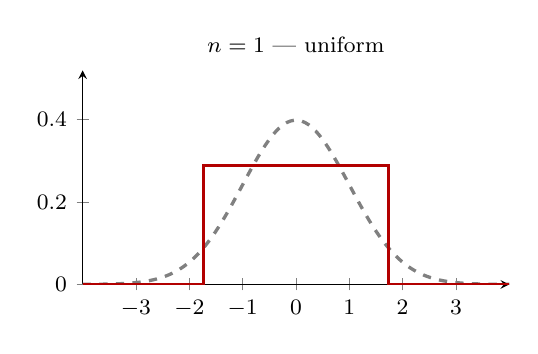
\begin{tikzpicture}
    \begin{axis}[
      title={$n = 1$ --- uniform},
      width=7.0cm, height=4.3cm,
      axis lines=left,
      xmin=-4, xmax=4, ymin=0, ymax=0.52,
      xtick={-3,-2,-1,0,1,2,3}, ytick={0,0.2,0.4},
      tick label style={font=\footnotesize},
      title style={font=\footnotesize, yshift=-3pt},
      every axis plot/.append style={very thick},
    ]
      \addplot[gray, dashed, domain=-4:4, samples=120]
        {0.3989423*exp(-x^2/2)};
      \addplot[red!70!black] coordinates
        {(-4,0) (-1.7321,0) (-1.7321,0.28868) (1.7321,0.28868)
         (1.7321,0) (4,0)};
    \end{axis}
  \end{tikzpicture}
  \hfill
  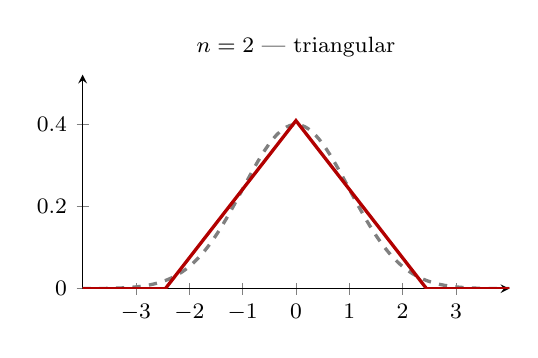
\begin{tikzpicture}
    \begin{axis}[
      title={$n = 2$ --- triangular},
      width=7.0cm, height=4.3cm,
      axis lines=left,
      xmin=-4, xmax=4, ymin=0, ymax=0.52,
      xtick={-3,-2,-1,0,1,2,3}, ytick={0,0.2,0.4},
      tick label style={font=\footnotesize},
      title style={font=\footnotesize, yshift=-3pt},
      every axis plot/.append style={very thick},
    ]
      \addplot[gray, dashed, domain=-4:4, samples=120]
        {0.3989423*exp(-x^2/2)};
      \addplot[red!70!black] coordinates
        {(-4,0) (-2.4495,0) (0,0.40825) (2.4495,0) (4,0)};
    \end{axis}
  \end{tikzpicture}

  \vspace{4mm}

  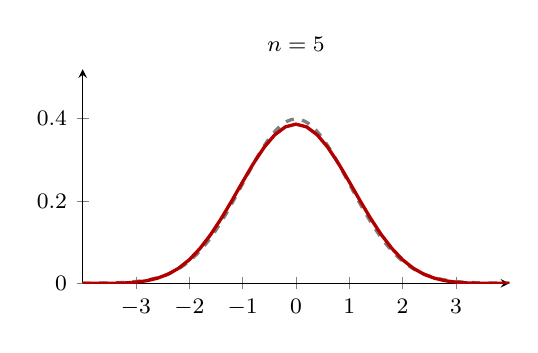
\begin{tikzpicture}
    \begin{axis}[
      title={$n = 5$},
      width=7.0cm, height=4.3cm,
      axis lines=left,
      xmin=-4, xmax=4, ymin=0, ymax=0.52,
      xtick={-3,-2,-1,0,1,2,3}, ytick={0,0.2,0.4},
      tick label style={font=\footnotesize},
      title style={font=\footnotesize, yshift=-3pt},
      every axis plot/.append style={very thick},
    ]
      \addplot[gray, dashed, domain=-4:4, samples=120]
        {0.3989423*exp(-x^2/2)};
      \addplot[red!70!black] coordinates {
        (-4.0,0.0) (-3.8,0.0) (-3.6,0.00003) (-3.4,0.00023) (-3.2,0.00096) (-3.0,0.00271)
        (-2.8,0.00619) (-2.6,0.01226) (-2.4,0.02198) (-2.2,0.03657) (-2.0,0.05721) (-1.8,0.08447)
        (-1.6,0.11823) (-1.4,0.15764) (-1.2,0.20113) (-1.0,0.24642) (-0.8,0.29052) (-0.6,0.32974)
        (-0.4,0.36045) (-0.2,0.37995) (0.0,0.38663) (0.2,0.37995) (0.4,0.36045) (0.6,0.32974)
        (0.8,0.29052) (1.0,0.24642) (1.2,0.20113) (1.4,0.15764) (1.6,0.11823) (1.8,0.08447)
        (2.0,0.05721) (2.2,0.03657) (2.4,0.02198) (2.6,0.01226) (2.8,0.00619) (3.0,0.00271)
        (3.2,0.00096) (3.4,0.00023) (3.6,0.00003) (3.8,0.0) (4.0,0.0)};
    \end{axis}
  \end{tikzpicture}
  \hfill
  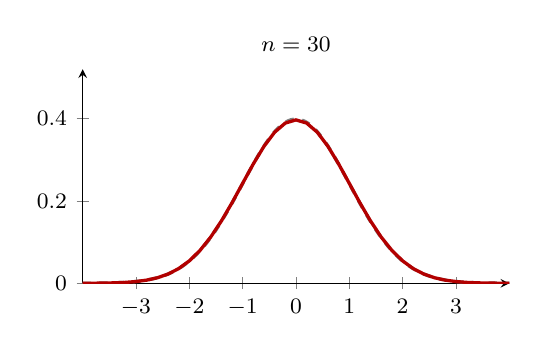
\begin{tikzpicture}
    \begin{axis}[
      title={$n = 30$},
      width=7.0cm, height=4.3cm,
      axis lines=left,
      xmin=-4, xmax=4, ymin=0, ymax=0.52,
      xtick={-3,-2,-1,0,1,2,3}, ytick={0,0.2,0.4},
      tick label style={font=\footnotesize},
      title style={font=\footnotesize, yshift=-3pt},
      every axis plot/.append style={very thick},
    ]
      \addplot[gray, dashed, domain=-4:4, samples=120]
        {0.3989423*exp(-x^2/2)};
      \addplot[red!70!black] coordinates {
        (-4.0,0.0001) (-3.8,0.00023) (-3.6,0.00052) (-3.4,0.00109) (-3.2,0.00219) (-3.0,0.0042)
        (-2.8,0.00768) (-2.6,0.01339) (-2.4,0.02233) (-2.2,0.03563) (-2.0,0.05445) (-1.8,0.07975)
        (-1.6,0.11202) (-1.4,0.15097) (-1.2,0.19534) (-1.0,0.24278) (-0.8,0.28989) (-0.6,0.33267)
        (-0.4,0.36699) (-0.2,0.38924) (0.0,0.39694) (0.2,0.38924) (0.4,0.36699) (0.6,0.33267)
        (0.8,0.28989) (1.0,0.24278) (1.2,0.19534) (1.4,0.15097) (1.6,0.11202) (1.8,0.07975)
        (2.0,0.05445) (2.2,0.03563) (2.4,0.02233) (2.6,0.01339) (2.8,0.00768) (3.0,0.0042)
        (3.2,0.00219) (3.4,0.00109) (3.6,0.00052) (3.8,0.00023) (4.0,0.0001)};
    \end{axis}
  \end{tikzpicture}
\end{figure}

\begin{example}[Fluctuations of a Bernoulli frequency]
  Soit $X_{1}, X_{2}, \dots$ une suite de variables aléatoires i.i.d.\ suivant
  une loi de Bernoulli $\mathcal{B}(p)$ de paramètre
  $p \in [0,1]$. The variance is $p(1-p)$, so
  \[
    \sqrt{n}\left(\frac{1}{n}\sum_{i=1}^{n} X_{i} - p\right)
      \cvL \mathcal{N}(0, p(1-p)) .
  \]
  Autrement dit, pour $n$ assez grand, la loi de l'écart de la moyenne
  empirique à la valeur limite $p$ est proche d'une loi normale centrée et de
  variance $p(1-p)/n$.
  This is the statement behind every confidence interval for a proportion.
\end{example}

\begin{example}[A loi du $\chi^{2}$ is asymptotically normal]
  La loi du $\chi^{2}$ à $n$ degrés de liberté is by definition the loi of
  $Z_{1}^{2} + \cdots + Z_{n}^{2}$ with $Z_{1}, \dots, Z_{n}$ i.i.d.\
  $\mathcal{N}(0,1)$. The summands are i.i.d.; comme
  $\expec(Z_{1}^{2}) = 1$ et
  $\Var(Z_{1}^{2}) = \expec(Z_{1}^{4}) - 1 = 3 - 1 = 2$, both finite, the
  théorème central limite applies to them. Formellement,
  \[
    \frac{1}{\sqrt{n}}\left(\sum_{i=1}^{n} Z_{i}^{2} - n\right)
      \cvL \mathcal{N}(0,2) .
  \]
  La loi $\chi^{2}(n)$ est donc proche de $\mathcal{N}(n, 2n)$, pourvu que $n$
  soit assez grand. The moment $\expec(Z_{1}^{4}) = 3$ is the moment d'ordre 4
  of the loi normale centrée réduite, read off the fourth-order expansion of
  $e^{-t^{2}/2}$ in the fonction caractéristique chapter.
\end{example}

\begin{example}[A Poisson sum cut at its mean]
  For $a, n > 0$ set $F(a,n) = \sum_{k=0}^{\lfloor an \rfloor} n^{k}/k!$. Since
  a sum of $n$ i.i.d.\ $\mathcal{P}(1)$ variables follows $\mathcal{P}(n)$ ---
  which the fonction génératrice settles in one line, $G_{Y}(s) = e^{n(s-1)} =
  (e^{s-1})^{n}$ --- one may write $e^{-n}F(a,n) = \prob(Y \leq an)$ with
  $Y \sim \mathcal{P}(n)$, that is, $Y = X_{1} + \cdots + X_{n}$ for i.i.d.\
  $\mathcal{P}(1)$ variables.\\
  For $a \in (0,1)$, the loi forte gives
  $\frac{1}{n}(X_{1} + \cdots + X_{n}) \cvas 1$, hence convergence en loi to
  the constant $1$, whose fonction de répartition is continuous at
  $a < 1$; therefore $e^{-n}F(a,n) = \prob(\frac{1}{n}\sum X_{i} \leq a) \to 0$.\\
  At the critical value $a = 1$ the loi forte says nothing, since $1$ is the
  discontinuity point of the limit, and the théorème central limite takes over:
  $\sqrt{n}(\frac{1}{n}\sum X_{i} - 1) \cvL \mathcal{N}(0,1)$ because
  $\mathcal{P}(1)$ has espérance and variance both equal to $1$, and $0$ is a
  continuity point of the fonction de répartition of the loi normale, so
  \[
    e^{-n}F(1,n) = \prob\!\left(\sqrt{n}\left(\tfrac{1}{n}\textstyle\sum_{i} X_{i}
      - 1\right) \leq 0\right) \; \longrightarrow \; \frac{1}{2} .
  \]
  The example is the clearest illustration of the division of labour between the
  two theorems: away from the mean the loi forte decides, and exactly at the
  mean only the théorème central limite can.
\end{example}

\begin{example}[Fluctuations of the limiting geometric mean]
  Continuing the uniform example of the previous subsection, with
  $G_{n} = \sqrt[n]{U_{1}\cdots U_{n}}$ and $\expec(\ln U_{1}) = -1$. Set
  $Z_{n} = (c\,G_{n})^{\sqrt{n}}$ and take a logarithm:
  \[
    \ln Z_{n} = \sqrt{n}\left(\ln c + \frac{1}{n}\sum_{i=1}^{n} \ln U_{i}\right) .
  \]
  This is the théorème central limite's expression provided $\ln c$ cancels the
  espérance, that is $\ln c = -\expec(\ln U_{1}) = 1$, so $c = e$. Since
  $-\ln U_{1} \sim \mathcal{E}(1)$ has variance $1$,
  \[
    \ln Z_{n} \cvL \mathcal{N}(0,1) ,
  \]
  and the exponential being continuous, $Z_{n} \cvL Z = e^{X}$ with
  $X \sim \mathcal{N}(0,1)$. The densité of $Z$ follows from the théorème de
  transfert and the changement de variable $z = e^{x}$. Pour toute fonction
  mesurable $\phi \geq 0$,
  \[
    \expec(\phi(Z)) = \int_{\reals} \phi(e^{x})
      \frac{1}{\sqrt{2\pi}} e^{-x^{2}/2} dx
    = \int_{0}^{+\infty} \phi(z) \frac{1}{\sqrt{2\pi}\,z}
      e^{-(\ln z)^{2}/2} \, dz ,
  \]
  la densité est donc :
  \[
    f_{Z}(z) = \frac{1}{\sqrt{2\pi}\,z} e^{-(\ln z)^{2}/2}
      \indic_{\reals_{+}}(z) ,
  \]
  c'est une \textbf{loi log-normale} (\textit{log-normal distribution}). Between
  them, this example and the one it continues use both stability results of the
  first two subsections, in the same shape --- the presque sûre one there, the
  one for convergence en loi here:
  the logarithm turns the product into a sum, the limit theorem acts on the sum,
  the exponential carries the conclusion back.
\end{example}

\begin{example}[Excess of ones over zeros in a binary expansion]
  Soit $U$ une variable aléatoire uniforme sur $[0,1]$. On note $X_{n}$ et
  $Y_{n}$ les nombres de 0 et de 1 parmi les $n$ premiers bits de sa
  décomposition binaire. With
  $b_{1}, b_{2}, \dots$ i.i.d.\ of loi $\mathcal{B}(1/2)$ as before,
  $Y_{n} = \sum_{k \leq n} b_{k}$ and $X_{n} = n - Y_{n}$, so
  \[
    X_{n} - Y_{n} = \sum_{k=1}^{n} (1 - 2b_{k}) .
  \]
  The summands $1 - 2b_{k}$ are i.i.d., take the values $\pm 1$ with probability
  $1/2$ each, and so have espérance $0$ and variance $1$. The specialised form
  of the théorème central limite applies directly:
  \[
    \frac{X_{n} - Y_{n}}{\sqrt{n}} \cvL \mathcal{N}(0,1) .
  \]
  The loi forte already said that the excess is $o(n)$; the théorème central
  limite says it is of order exactly $\sqrt{n}$, with Gaussian fluctuations.
\end{example}

\begin{example}[A rate the théorème central limite does not supply]
  The théorème central limite is a statement about a limit and gives no bound at
  any fixed $n$. When a bound is wanted --- an \textbf{inégalité de déviation}
  (\textit{deviation inequality}) --- the route is the exponential moment, and
  it is worth carrying because the technique reappears whenever a rate is asked
  for.\\
  Let $Y_{1}, Y_{2}, \dots$ be i.i.d.\ on $\{-1,+1\}$ with
  $\prob(Y_{1} = 1) = 1/2$, and $S_{n} = Y_{1} + \cdots + Y_{n}$. Fix $a > 0$.
  \begin{enumerate}
    \item \emph{Exponentiate, then apply Markov.} For every $x > 0$ the map
      $s \mapsto e^{xs}$ is increasing, so $\{S_{n} > a\} = \{e^{xS_{n}} >
      e^{xa}\}$, and the inégalité de Markov applied to the non-negative
      variable $e^{xS_{n}}$ gives $\prob(S_{n} > a) \leq e^{-ax}\expec(e^{xS_{n}})$.
    \item \emph{Compute the exponential moment.} The variables being
      indépendantes et identiquement distribuées,
      $\expec(e^{xS_{n}}) = \expec(e^{xY_{1}})^{n} = \cosh(x)^{n}$, since
      $\expec(e^{xY_{1}}) = \frac{1}{2}(e^{x} + e^{-x})$.
    \item \emph{Bound it.} Studying the sign of $x \mapsto x^{2}/2 -
      \ln\cosh(x)$, whose derivative $x - \tanh(x)$ is non-negative on
      $\reals_{+}$ and which vanishes at $0$, gives $\cosh(x) \leq e^{x^{2}/2}$,
      hence $\expec(e^{xS_{n}}) \leq e^{nx^{2}/2}$ for $x > 0$.
    \item \emph{Optimise.} The bound is now $e^{-ax + nx^{2}/2}$; minimising the
      exponent over $x > 0$ gives $x = a/n$ and
      $\prob(S_{n} > a) \leq e^{-a^{2}/(2n)}$.
    \item \emph{Symmetrise.} The loi of $S_{n}$ is symétrique, so the borne de
      l'union gives $\prob(|S_{n}| > a) \leq 2e^{-a^{2}/(2n)}$.
  \end{enumerate}
  Two things to notice. The bound holds at every $n$, not asymptotically, which
  is what the limit theorems never give. And taking $a = \varepsilon n$ gives
  $\prob(|S_{n}/n| > \varepsilon) \leq 2e^{-\varepsilon^{2}n/2}$, an exponential
  rate for a convergence that the loi forte, read through the implication of
  the first subsection, gives without any rate at all.
\end{example}

\subsection{Cas des vecteurs aléatoires}
La loi des grands nombres et le théorème central limite s'étendent sans
difficulté au cas vectoriel. The empirical mean is taken coordinate by
coordinate, the espérance becomes a vector, and the variance becomes a matrice
de covariance $\Gamma$.

\begin{theorem}[Loi forte des grands nombres -- cas vectoriel]
  Pour toute suite $X_{1}, X_{2}, \dots$ de vecteurs aléatoires réels
  i.i.d.\ \emph{ayant une espérance},
  \[
    \frac{1}{n} \sum_{i=1}^{n} X_{i} \cvas \expec(X_{1}) .
  \]
\end{theorem}

\begin{theorem}[Théorème central limite -- cas vectoriel]
  Pour toute suite $X_{1}, X_{2}, \dots$ de vecteurs aléatoires réels i.i.d.\
  d'espérance finie $\mu$ et de matrice de covariance finie $\Gamma$,
  \[
    \sqrt{n}\left(\frac{1}{n}\sum_{i=1}^{n} X_{i} - \mu\right)
      \cvL \mathcal{N}(0, \Gamma) .
  \]
\end{theorem}

\begin{remark}
  The loi forte in the vector case is the scalar one applied to each
  coordinate, together with the fact that a finite intersection of événements
  of probability $1$ has probability $1$ --- which is why it costs nothing. The
  théorème central limite in the vector case is genuinely more than its
  coordinates: convergence en loi of each coordinate does not give convergence
  en loi of the vector, since the loi jointe is not determined by the lois
  marginales. What repairs this is the fonction caractéristique of a vecteur
  aléatoire, which does determine the loi jointe, together with the vector form
  of branch 3: pointwise convergence of fonctions caractéristiques on
  $\reals^{d}$, $d$ being the dimension of the vectors, gives convergence en
  loi. That vector form is the missing ingredient and is stated, not proved,
  here --- the characterisation theorem above is for variables aléatoires
  réelles, and this course states the vector case without supplying it. The
  matrice de covariance
  $\Gamma$ carries the dependence between coordinates that the lois marginales
  lose.
\end{remark}

\begin{remark}
  ``Matrice de covariance finie'' means every entry finite, that is, a moment
  d'ordre $2$ for every coordinate. No invertibility of $\Gamma$ is required
  anywhere: a $\Gamma$ that is dégénérée gives a vecteur gaussien supported on
  a proper subspace, which is a perfectly good limit en loi even though it has
  no densité on $\reals^{d}$.
\end{remark}

\begin{example}[Uniform points on the unit disc]
  Soit $X_{1}, X_{2}, \dots$ une suite de vecteurs aléatoires réels i.i.d.\ (in
  $\reals^{2}$) de loi uniforme sur le disque unité. Their espérance is $0$ by
  symmetry, and leur matrice de covariance est $I/4$, où $I$ désigne la matrice
  identité en dimension $2$: writing
  $X_{1} = (X, Y)$ for the two coordinates of one point, the off-diagonal entry
  $\expec(XY)$ vanishes by symmetry, and in polar coordinates the diagonal entry
  is
  \[
    \expec(X^{2}) = \frac{1}{\pi}\int_{0}^{2\pi}\!\!\int_{0}^{1}
      r^{2}\cos^{2}\theta \cdot r \, dr \, d\theta
    = \frac{1}{\pi} \cdot \frac{1}{4} \cdot \pi = \frac{1}{4} .
  \]
  Alors, by the théorème central limite in the vector case,
  \[
    \sqrt{n}\left(\frac{1}{n}\sum_{i=1}^{n} X_{i}\right)
      \cvL \mathcal{N}\!\left(0, \frac{I}{4}\right) .
  \]
  The limit is a rescaled vecteur gaussien centré réduit, so its level sets are
  circles: the isotropy of the disc survives into the limit.
\end{example}

\begin{example}[The barycentre of random points]
  Soit $G_{n}$ le barycentre de $n$ points aléatoires indépendants de même loi
  uniforme sur le disque unité. Then $G_{n} = \frac{1}{n}\sum_{i \leq n} X_{i}$
  is exactly the empirical mean of the previous example, so $G_{n} \cvas 0$ by
  the loi forte in the vector case, and
  \[
    \sqrt{n}\, G_{n} \cvL \mathcal{N}\!\left(0, \frac{I}{4}\right) .
  \]
  The barycentre of many random points is near the centre, at distance of order
  $1/\sqrt{n}$, and its fluctuation is isotropic Gaussian.
\end{example}

\begin{example}[Order statistics of two uniform variables]
  Soient $U, V$ deux variables aléatoires indépendantes de loi uniforme sur
  $[0,1]$. On note le vecteur
  $Z = (X, Y)$ avec $X = \min(U,V)$ et $Y = \max(U,V)$, et
  $Z_{1}, Z_{2}, \dots$ une suite de vecteurs aléatoires i.i.d.\ de même loi
  que $Z$.\\
  \emph{The loi of $Z$.} The pair $(U,V)$ has densité $\indic_{[0,1]^{2}}$, and
  $(X,Y)$ is obtained by folding the square along its diagonal --- the two
  points $(u,v)$ and $(v,u)$ give the same $(x,y)$ --- so
  \[
    f_{Z}(x,y) = 2 \, \indic_{\{0 < x < y < 1\}} .
  \]
  \emph{The almost-sure limit.} The lois marginales have densités $2(1-x)$ and
  $2y$ on $[0,1]$, so $\expec(X) = 1/3$ and $\expec(Y) = 2/3$, and the loi
  forte in the vector case gives
  \[
    \frac{1}{n}\sum_{k=1}^{n} Z_{k} \cvas \mu = \left(\frac{1}{3},
      \frac{2}{3}\right) .
  \]
  \emph{The fluctuations.} The second moments are $\expec(X^{2}) = 1/6$ and
  $\expec(Y^{2}) = 1/2$, so $\Var(X) = \Var(Y) = 1/18$; and since
  $XY = UV$ with $U, V$ independent, $\expec(XY) = 1/4$ and
  $\Cov(X,Y) = 1/4 - 2/9 = 1/36$. Hence
  \[
    \Gamma = \frac{1}{36}\begin{pmatrix} 2 & 1 \\ 1 & 2 \end{pmatrix} ,
    \qquad
    \sqrt{n}\left(\frac{1}{n}\sum_{k=1}^{n} Z_{k} - \mu\right)
      \cvL \mathcal{N}(0, \Gamma) .
  \]
  The off-diagonal entry is positive and non-zero, as it must be --- the minimum
  and the maximum of the same pair move together --- and this is exactly the
  information that treating the two coordinates separately would have thrown
  away.
\end{example}

\begin{conclusion}
  Two notions of convergence, two theorems, one bridge between them. Convergence
  presque sûre is pointwise convergence on an événement of probability $1$, and
  everything true of convergent sequences of reals transfers to it by
  intersecting such événements. Convergence en loi looks only at the
  lois, through
  fonctions de répartition at continuity points of the limit, and is
  equivalently tested on bounded continuous functions or, decisively, on
  fonctions caractéristiques --- which lets a loi limite be identified by a
  computation with no univers in it. Convergence presque sûre implies it,
  through convergence en probabilité if that mode is carried, and nothing
  implies convergence presque sûre.\\
  The loi forte needs an espérance and delivers an almost-sure limit; the
  théorème central limite needs a variance as well, delivers only a limit en
  loi, and in exchange describes the deviation at the scale $\sqrt{n}$ with a
  Gaussian whose covariance is the only trace the underlying loi
  leaves. In
  practice the two are used in sequence and on transformed sequences: take a
  logarithm to turn a product into a sum, apply the loi forte for the location
  and the théorème central limite for the fluctuation, and push both conclusions
  back through a continuous map.
\end{conclusion}
